\chapter{Polynomial and Rational Inequalities}

\section{Polynomial Inequalities}

\section{Rational Inequalities}

When solving rational inequalities, you will need to find the critical values for your number line. To do so,

\begin{itemize}
    \item Find the domain restrictions (like in Graphs of Rational Functions)
    \item Solve the inequality as an equation (might want to multiply both sides by least common denominator)
\end{itemize}

We will test each of these critical values in the original problem and see if they make the original inequality true. \newline 

\begin{example}
Solve each.
\begin{multicols}{3}
\begin{enumerate}[(a)]
    \item $\frac{x+3}{x-2} \leq 0$
    \item $\frac{2x^2 - 3x - 5}{x^2 - 5x - 6} \geq 0$
    \item $\frac{x+7}{3x-1} < 4$
\end{enumerate}
\end{multicols}
\end{example}

\begin{solution}

(a) First, the domain:

\begin{align*}
    x - 2 &\neq 0 \\
    x &\neq 2
\end{align*}

Next, the solution as an equation:

\begin{align*}
    \frac{x+3}{x-2} &= 0 \\
    x + 3 &= 0 \qquad \text{multiply both sides by the denominator} \\
    x &= -3 
\end{align*}

We can set up a number line with these 2 critical values (2 and $-3$):

\begin{center}
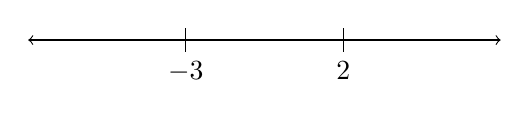
\begin{tikzpicture}
\draw [<->] (0,0) -- (6,0);
\draw (2,0.15) -- (2,-0.15) node [below] {$-3$};
\draw (4,0.15) -- (4,-0.15) node [below] {$2$};
\end{tikzpicture}
\end{center}

Next, we want to use \textit{test values} in each interval; as well as at the critical values against whether or not the outputs at those values are less than or equal to 0.

\begin{center}
\setlength{\extrarowheight}{4pt}
\begin{tabular}{c|c}
    $x$ & $\frac{x+3}{x-2} \leq 0$? \\ \hline
    $-4$ & $\frac{1}{6}$ (no) \\[5pt] 
    $-3$ & 0 (yes) \\[5pt]
    0 & $-\frac{3}{2}$ (yes) \\[5pt]
    2 & undefined (no) \\[5pt]
    3 & 6 (no) 
\end{tabular}
\end{center}

These results yield the following number line:

\begin{center}
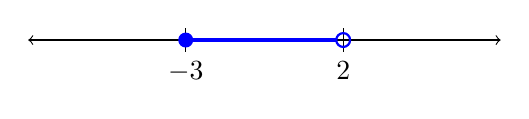
\begin{tikzpicture}
\draw [<->] (0,0) -- (6,0);
\draw (2,0.15) -- (2,-0.15) node [below] {$-3$};
\draw (4,0.15) -- (4,-0.15) node [below] {$2$};
\draw [blue, fill=blue] (2,0) circle [radius = 2.5pt];
\draw [blue, thick] (4,0) circle [radius = 2.5pt];
\draw [ultra thick, blue, shorten <= 2.5pt, shorten >= 2.5pt] (2,0) -- (4,0);
\end{tikzpicture}
\end{center}

In interval notation, our solution is $[-3, 2)$. \\[18pt]

(b) First, the domain:

\begin{align*}
    x^2 - 5x - 6 &\neq 0 \\
    (x - 6)(x + 1) &\neq 0 \\
    x-6\neq 0 &\text{ and } x + 1 \neq 0 \\
    x \neq 6 &\text{ and } x \neq -1 
\end{align*}

Next, the solution as an equation:

\begin{align*}
    \frac{2x^2-3x-5}{x^2-5x-6} &= 0 \\
    2x^2 - 3x - 5 &= 0 \qquad \text{multiply both sides by the denominator} \\
    (2x - 5)(x + 1) &= 0 \\
    2x - 5 = 0 &\text{ or } x + 1 = 0 \\
    x = \tfrac{5}{2} &\text{ or } x = -1
\end{align*}

\bigskip 

We have 3 distinct critical values: $-1$, $\tfrac{5}{2}$, and 6. \newline 

\begin{center}
\begin{tikzpicture}
    \draw [<->] (0,0) -- (6,0);
    \draw (1.5,0.15) -- (1.5,-0.15) node [below] {$-1$};
    \draw (3, 0.15) -- (3, -0.15) node [below] {$\tfrac{5}{2}$};
    \draw (4.5, 0.15) -- (4.5, -0.15) node [below] {6};
\end{tikzpicture}
\end{center}

We then check the critical values in the original inequality, along with other test values:

\begin{center}
\setlength{\extrarowheight}{4pt}
\begin{tabular}{c|c}
    $x$ & $\frac{2x^2-3x-5}{x^2-5x-6} \geq 0$? \\ \hline 
    $-2$ & $\tfrac{9}{8}$ (yes) \\
    $-1$ & undefined (no) \\
    0 & $\tfrac{5}{6}$ (yes) \\
    $\tfrac{5}{2}$ & 0 (yes) \\
    3 & $-\tfrac{1}{3}$ (no) \\
    6 & undefined (no) \\
    7 & 9 (yes) 
\end{tabular}
\end{center}

\begin{center}
\begin{tikzpicture}
    \draw [<->] (0,0) -- (6,0);
    \draw (1.5,0.15) -- (1.5,-0.15) node [below] {$-1$};
    \draw (3, 0.15) -- (3, -0.15) node [below] {$\tfrac{5}{2}$};
    \draw (4.5, 0.15) -- (4.5, -0.15) node [below] {6};
    \draw [blue, thick] (1.5,0) circle [radius = 2.5pt];
    \draw [blue, fill=blue] (3,0) circle [radius = 2.5pt];
    \draw [blue, thick, fill=blue] (4.5,0) circle [radius = 2.5pt];
    \draw [->, blue, ultra thick, shorten <= 2.5pt] (1.5,0) -- (0,0);
    \draw [blue, ultra thick, shorten <= 2.5pt, shorten >= 2.5pt] (1.5,0) -- (3,0);
    \draw [->, blue, ultra thick, shorten <= 2.5pt] (4.5,0) -- (6,0);
\end{tikzpicture}
\end{center}

In interval notation, our solution is $(-\infty, -1) \cup \left(-1, \tfrac{5}{2}\right] \cup [6, \infty)$ \\[18pt]

(c) First, the domain:
\begin{align*}
    3x - 1 &\neq 0 \\
    x &\neq \tfrac{1}{3}
\end{align*}

Next, the solution to the inequality as an equation:
\begin{align*}
    \frac{x+7}{3x-1} &= 4 \\
    x+7 &= 4(3x-1) \qquad \text{multiply both sides by the denominator} \\
    x + 7 &= 12x - 4 \\
    x &= 1
\end{align*}

Our number line looks like

\begin{center}
\begin{tikzpicture}
\draw [<->] (0,0) -- (6,0);
\draw (2,0.15) -- (2,-0.15) node [below] {$\tfrac{1}{3}$};
\draw (4, 0.15) -- (4,-0.15) node [below] {1};
\end{tikzpicture}
\end{center}

Testing the critical values and others in the original inequality:

\begin{center}
\setlength{\extrarowheight}{4pt}
\begin{tabular}{c|c}
    $x$ & $\frac{x+7}{3x-1} < 4$ ? \\ \hline 
    0 & $-7$ (yes) \\
    $\tfrac{1}{3}$ & undefined (no) \\
    $\tfrac{1}{2}$ & 15 (no) \\
    1 & 4 (no) \\
    2 & $\tfrac{9}{5}$ (yes)
\end{tabular}
\end{center}

\begin{center}
\begin{tikzpicture}
\draw [<->] (0,0) -- (6,0);
\draw (2,0.15) -- (2,-0.15) node [below] {$\tfrac{1}{3}$};
\draw (4, 0.15) -- (4,-0.15) node [below] {1};
\draw [->, ultra thick, shorten <= 2.5pt, blue] (2,0) -- (0,0);
\draw [blue, thick] (2,0) circle [radius = 2.5pt];
\draw [blue, thick] (4,0) circle [radius = 2.5pt];
\draw [->, blue, ultra thick, shorten <= 2.5pt] (4,0) -- (6,0);
\end{tikzpicture}
\end{center}
 
In interval notation, our solution is $\left(-\infty, \tfrac{1}{3}\right) \cup (1, \infty)$ 
\end{solution}

%{\color{red}{\color{red}\textbf{Exercise.}}} Solve each.
%
%\begin{multicols}{3}
%\begin{enumerate}[(a)]
%    \item $\frac{2x-4}{x-7} > 0$
%    \item $\frac{x^2 - 6x - 27}{3x^2 - 25x + 28} \leq 0$
%    \item $\frac{5x+7}{2x+3} \geq 2$
%\end{enumerate}
%\end{multicols}

\section{Exercises}

\subsection*{Polynomial Inequalities}

Solve each. Write your answers using interval notation.
\begin{multicols}{2}
\begin{enumerate}
\item $6x^3-4x^2-10x \geq 0$
\item $x^4 < 9x^2$
\end{enumerate} \setcounter{Review}{\value{enumi}}
\end{multicols}
\begin{multicols}{2}
\begin{enumerate}	\setcounter{enumi}{\value{Review}}
\item $3x^3-7x^2-22x+8 < 0$
\item $3x^2 - 4x + 1 \leq 0$
\end{enumerate} \setcounter{Review}{\value{enumi}}
\end{multicols}
\begin{multicols}{2}
\begin{enumerate}	\setcounter{enumi}{\value{Review}}
\item $12x^4 + 76x^3 + 43x^2 - 346x - 280 \geq 0$
\item $-2x^4 + 49x^2 + 21x^3 - 1029x + 2401 \geq 0$
\end{enumerate} \setcounter{Review}{\value{enumi}}
\end{multicols}
\begin{multicols}{2}
\begin{enumerate}	\setcounter{enumi}{\value{Review}}
\item $-x^2 - 7x - 6 \leq 0$
\item $x^2 + 4x + 4 < 0$
\end{enumerate} \setcounter{Review}{\value{enumi}}
\end{multicols}
\begin{multicols}{2}
\begin{enumerate}	\setcounter{enumi}{\value{Review}}
\item $-x^4 - 6x^3 + 61x^2 + 234x - 1008 \geq 0$
\item $-x^2 + 3x + 1 > 3$
\end{enumerate} \setcounter{Review}{\value{enumi}}
\end{multicols}
\begin{multicols}{2}
\begin{enumerate}	\setcounter{enumi}{\value{Review}}
\item $-3x^4 + 123x^3 + 142x^2 - 424x + 320 \leq 122x^3$
\item $-x^4 - 1120 + 77x^2 - 36x + 15x^3 \geq 15x^3$
\end{enumerate} \setcounter{Review}{\value{enumi}}
\end{multicols}
\begin{multicols}{2}
\begin{enumerate}	\setcounter{enumi}{\value{Review}}
\item $-3x^4 - 22x^3 + 271x^2 + 152x - 96 \geq 267x^2$
\item $15x^3 + 27x^2 + 8x \leq 14x$
\end{enumerate}	\setcounter{Review}{\value{enumi}}
\end{multicols}
\begin{multicols}{2}
\begin{enumerate}	\setcounter{enumi}{\value{Review}}
\item $x^3 + 6x^2 > -2x^2 + 64x + 512$

\end{enumerate}	\setcounter{enumi}{\value{Review}}
\end{multicols}

\subsection*{Domain}
State the domain of each. Write your answers using interval notation.
\begin{enumerate}	\setcounter{Review}{\value{enumi}}
\item $b(x) = \sqrt{21x^2 - 23x - 20}$
\item $f(x) = \frac{3}{\sqrt{3x^2 + 2x - 1}}$
\item $g(x) = \sqrt[4]{2x^3+9x^2+12x+4}$
\end{enumerate}	\setcounter{enumi}{\value{Review}}

\subsection*{Rational Inequalities}
Solve each. Write your answers using interval notation.
\begin{multicols}{3}
\begin{enumerate}	\setcounter{Review}{\value{enumi}}
\setlength\itemsep{10pt}
\item $\frac{3x-4}{x+1}<0$
\item $\frac{x^2+3x+2}{x-7} \leq 0$
\item $\frac{x^2-4x+4}{x^2-1} \geq 0$
\end{enumerate} \setcounter{Review}{\value{enumi}}
\end{multicols}
\begin{multicols}{3}
\begin{enumerate}	\setcounter{enumi}{\value{Review}}
\item $\frac{x+2}{x-4} \leq 1$
\item $\frac{x^2-7x-8}{x^2-4x-32} \geq 0$
\item $\frac{4+3x}{5-x} \leq 2$
\end{enumerate} \setcounter{Review}{\value{enumi}}
\end{multicols}
\begin{multicols}{3}
\begin{enumerate}	\setcounter{enumi}{\value{Review}}
\item $\frac{x-4}{x+7} < 0$
\item $\frac{x+5}{x+7} < 0$
\item $\frac{2x-26}{5x+20} > -3$
\end{enumerate} \setcounter{Review}{\value{enumi}}
\end{multicols}
\begin{multicols}{3}
\begin{enumerate}	\setcounter{enumi}{\value{Review}}
\item $\frac{2x-50}{5x+15} \leq -1$
\item $\frac{x+5}{x^2-2x-15} \leq 0$
\item $-\frac{2}{x} \geq - \frac{3}{x+1}$
\end{enumerate} \setcounter{Review}{\value{enumi}}
\end{multicols}
\begin{multicols}{3}
\begin{enumerate}	\setcounter{enumi}{\value{Review}}
\item $-\frac{3}{x+6} > -\frac{4}{x+7}$
\item $\frac{2x^2+3x-2}{x^2+5x+6} < 0$
\item $\frac{x-4}{2x+4} \geq 1$
\end{enumerate}	\setcounter{Review}{\value{enumi}}
\end{multicols}
\begin{multicols}{3}
\begin{enumerate}	\setcounter{enumi}{\value{Review}}
\item $\frac{6x^2+5x-21}{x-4} < 0$
\item $\frac{2x+1}{4x-3} \geq x-1$
\end{enumerate}	\setcounter{Review}{\value{enumi}}
\end{multicols}

\newpage

\section{Answer Key}

\section*{Polynomial Inequalities}
\begin{multicols}{2}
\begin{enumerate}
    \item $[-1,0] \cup \left[\frac{5}{3}, \infty\right)$
    \item $(-3,0) \cup (0,3)$
\end{enumerate} \setcounter{Review}{\value{enumi}}
\end{multicols}
\begin{multicols}{2}
\begin{enumerate}	\setcounter{enumi}{\value{Review}}
    \item $(-\infty, -2) \cup \left(\frac{1}{3}, 4\right)$
    \item $\left[\frac{1}{3}, 1\right]$
\end{enumerate} \setcounter{Review}{\value{enumi}}
\end{multicols}
\begin{multicols}{2}
\begin{enumerate}	\setcounter{enumi}{\value{Review}}
    \item $(-\infty, -4] \cup \left[-\frac{7}{2},-\frac{5}{6}\right] \cup [2, \infty)$
    \item $\left[-7, \frac{7}{2}\right] \cup {7}$
\end{enumerate} \setcounter{Review}{\value{enumi}}
\end{multicols}
\begin{multicols}{2}
\begin{enumerate}	\setcounter{enumi}{\value{Review}}
    \item $(-\infty, -6] \cup [-1, \infty)$
    \item $\emptyset$
\end{enumerate} \setcounter{Review}{\value{enumi}}
\end{multicols}
\begin{multicols}{2}
\begin{enumerate}	\setcounter{enumi}{\value{Review}}
    \item $[-8,-7] \cup [3, 6]$
    \item $(1,2)$
\end{enumerate} \setcounter{Review}{\value{enumi}}
\end{multicols}
\begin{multicols}{2}
\begin{enumerate}	\setcounter{enumi}{\value{Review}}
    \item $(-\infty, -8] \cup \left[\frac{4}{3}, 2\right] \cup [5, \infty)$
    \item $[-8, -4] \cup [5, 7]$
\end{enumerate} \setcounter{Review}{\value{enumi}}
\end{multicols}
\begin{multicols}{2}
\begin{enumerate}	\setcounter{enumi}{\value{Review}}
    \item $[-6, -4] \cup \left[\frac{2}{3}, 2\right]$
    \item $(-\infty, -2] \cup \left[0, \frac{1}{5}\right]$
\end{enumerate}	\setcounter{Review}{\value{enumi}}
\end{multicols}
\begin{multicols}{2}
\begin{enumerate}	\setcounter{enumi}{\value{Review}}
    \item $(8, \infty)$
\end{enumerate}	\setcounter{Review}{\value{enumi}}
\end{multicols}

\section*{Domain}
\begin{enumerate}
	\item $\left(-\infty, -\frac{12}{21}\right] \cup \left[\frac{5}{3}, \infty\right)$
	\item $(-\infty, -1) \cup \left(\frac{1}{3}, \infty\right)$
	\item $\{-2\} \cup \left[-\frac{1}{2}, \infty\right)$
\end{enumerate}

\section*{Rational Inequalities}
\begin{multicols}{2}
\begin{enumerate}
    \item $\left(-1, \frac{4}{3}\right)$
    \item $(-\infty,-2] \cup [-1, 7)$
\end{enumerate} \setcounter{Review}{\value{enumi}}
\end{multicols}
\begin{multicols}{2}
\begin{enumerate}	\setcounter{enumi}{\value{Review}}
    \item $(-\infty, -1) \cup (1, \infty)$
    \item $(-\infty, 4)$
\end{enumerate} \setcounter{Review}{\value{enumi}}
\end{multicols}
\begin{multicols}{2}
\begin{enumerate}	\setcounter{enumi}{\value{Review}}
    \item $(-\infty, -4) \cup [-1, 8) \cup (8, \infty)$
    \item $(-\infty, 1.2] \cup (5, \infty)$
\end{enumerate} \setcounter{Review}{\value{enumi}}
\end{multicols}
\begin{multicols}{2}
\begin{enumerate}	\setcounter{enumi}{\value{Review}}
    \item $(-7, 4)$
    \item $(-7, -5)$
\end{enumerate} \setcounter{Review}{\value{enumi}}
\end{multicols}
\begin{multicols}{2}
\begin{enumerate}	\setcounter{enumi}{\value{Review}}
    \item $(-\infty, -4) \cup (-2, \infty)$
    \item $(-3, 5]$
\end{enumerate} \setcounter{Review}{\value{enumi}}
\end{multicols}
\begin{multicols}{2}
\begin{enumerate}	\setcounter{enumi}{\value{Review}}
    \item $(-\infty, -5] \cup (-3, 5)$
    \item $(-1, 0) \cup [2, \infty)$
\end{enumerate} \setcounter{Review}{\value{enumi}}
\end{multicols}
\begin{multicols}{2}
\begin{enumerate}	\setcounter{enumi}{\value{Review}}
    \item $(-7, -6) \cup (-3, \infty)$
    \item $(-3,-2) \cup \left(-2, \frac{1}{2}\right)$
\end{enumerate}	\setcounter{Review}{\value{enumi}}
\end{multicols}
\begin{multicols}{2}
\begin{enumerate}	\setcounter{enumi}{\value{Review}}
    \item $[-8, -2)$
    \item $\left(-\infty, -\frac{7}{3}\right) \cup \left(\frac{3}{2}, 4\right)$ 
\end{enumerate}	\setcounter{Review}{\value{enumi}}
\end{multicols}
\begin{multicols}{2}
\begin{enumerate}	\setcounter{enumi}{\value{Review}}
    \item $\left(-\infty, \frac{1}{4}\right] \cup \left(\frac{3}{4}, 2\right]$
\end{enumerate}	\setcounter{Review}{\value{enumi}}
\end{multicols}